\documentclass[letterpaper, 12pt]{article}
\usepackage[margin=1in]{geometry}
\usepackage{times}
\usepackage{setspace}
\usepackage{lipsum}
\usepackage{graphicx}
\usepackage{float}
\usepackage[font=footnotesize]{caption}
\graphicspath{ {../Images/} }

\begin{document}
\bibliographystyle{plain}

\begin{titlepage}
    \begin{center}
        \vspace*{1in}
        \Huge{\textbf{Mini Project 1}}
        
        \vspace{0.5in}
        \Large{Noah Schiro}\\
        \Large{Jason Swope}
        
        \vfill
        
        \normalsize{November 11th, 2023}
        
        \vspace{0.5in}
        
        \normalsize{EE456: Introduction to Neural Networks}
        
        \vspace{0.5in}
        
        \normalsize{Pennsylvania State University}
        
    \end{center}
\end{titlepage}

\newpage

\setlength{\parindent}{5ex}
\setstretch{2} 

\section{Introduction}
In this project, we aim to demonstrate the capabilities of a Multilayer Perceptron (MLP) trained using the backpropagation algorithm in classifying nonlinearly separable data. Additionally, we explore a more challenging scenario where the MLP may face difficulties in differentiating classes for similarly structured data.

The objective of this project is to learn how MLPs train using backpropagation by implementation backpropagation ourselves. We will additionally learn the efficacy and limitations of MLPs in seperating nonlinear boundaries between classes of data. 

As a demonstration of this understanding, we seek to provide the following deliverables:

\begin{enumerate}
\item A visualization of how MLP prediction error changes over each epoch. We are interested in the error on the training set as well as the validation set. 
\item A visualization of the test data as well as the class boundary that the model derives superimposed onto this image
\item The associated code for training, testing, evaluation, and visualization of the results.
\end{enumerate}

\section{Implementation}

\subsection{Underlying linear algebra and backpropagation algorithm}
While there are many implementations of backpropagation across the many machine learning libraries today, one that stands above the rest in terms of efficiency and simplicity is automatic gradient computation.

Automatics gradient, or autograd for short, automatically and efficiently calculates the gradients of any mathematical expression with respect to its input variables. Autograd frameworks streamline the process of computing gradients by dynamically building and traversing the computational graph during the forward pass. This not only alleviates the burden of manual gradient derivation but also enables the implementation of complex neural network architectures. All neural networks do are operations on tensors. If we keep track of these operations as we feed forward through the network and compute our loss, then when we compute gradients, we will will see how each parameter of a neural network needs to be tuned to minimize loss.

\begin{enumerate}
\item  First, we constructed a class that wraps a floating point number. This class, called Scalar, has additional features such as storing the computation graph for any given value as well as storing the gradient.
\item Next, we build a linear algebra library on top of this. Each value in any given tensor is a Scalar object. All of the usual operations on tensors are built out, including but not limited to addition, multiplication, and unary functions such as ReLU and tanh.
\item Finally, we create a neural network API. Neural networks are just wrappers around tensor objects and a specific sequence of operations with those tensors. Crucial to our goal, we created the "Linear" object, which functions as a typical fully connected neural network layer with biases for each output neuron. Also instrumental to any neural network interface is loss function. In our case, we chose mean squared error. In theory, for a classification task such as this one, we could have also done binary cross entropy. Finally, we created an "optimizer" this is just an object that keeps track of the parameters we actually want to change and have learn. Everytime we call "step" on the optimizer, we move the parameters by their stored gradients.
\end{enumerate}

All of these elements together create a lightweight framework through which we can train our model for the task at hand, though in theory, this framework could be used for nearly any task that requires simple neural networks.

\subsection{Model architecture, hyperparameters, training, and evaluation}

Our model architecture follows the given model architecture. The input layer has two neurons, there is one hidden layer with ten neurons, and the output function has one neuron. The activation function used was the hyperbolic tangent function as the directions instructed.

Some of the hyper parameters were given, and the rest were determined from testing. The given hyperparameters were the learning rate and the threshold. The learning rate was decreased linearly from 10\textsuperscript{-1} to 10\textsuperscript{-5}, and the threshold is 0.

The hyperparameters that were determined using testing were the number of epochs, batch size, and train/test split.  The batch size of 60 provided a good balance of training time with validation accuracy.  The number of epochs needed for each dataset was different.  Training for dataset 1 plateaued near 30 epochs, and optimization stopped after 50, so 50 epochs was chosen so the data was learned, but the risk of overfitting was minimized.  Training for dataset 2 plateaued near 45 iterations and optimization stopped after 75, so 75 iterations was chosen.  A default value of 30\% of datapoints was chosen  for the proportion of validation datapoints, whihc perfomred well in our testing.

We also implemented two heuristics to help our MLP learn the data most efficiently. The first is the weight initializations. We used a balance between small and large weights by randomly sampling from a uniform distribution in the range [-1, 1]. This means the weights will be small enough that they will not be driven into saturation, and large enough that the backpropogation algorithm will not be placed in a flat region around the origin of the error surface.
The second was normalizing the data.  For both of the input features we subtracted the mean and divided by the standard deviation. Figures 1 shows a plot DataSet1 before and after nromalization, and Firgure 2 shows the same for DataSet2.

\begin{figure}
\centering
\includegraphics[scale = 0.5]{DataSet1Plot}
\includegraphics[scale = 0.5]{DataSet1NormalizedPlot}
\caption{Plot of DataSet1 (Left) and Plot of DataSet1 after Normalization (Right)}
\end{figure}
\begin{figure}
\centering
\includegraphics[scale = 0.5]{DataSet2Plot}
\includegraphics[scale = 0.5]{DataSet2NormalizedPlot}
\caption{Plot of DataSet2 (Left) and Plot of DataSet2 after Normalization (Right)}
\end{figure}

\section{Results}

The MLP performed very well on both datasets. The models recieved a final validation accuracy of 98.11\% and an average validation error\footnote{The average validation error is calculated by finding the sum of the mean squared errors of the validation data and dividing by the number of validation data points} of 0.059 on DataSet1, and a final validation accuracy of 98.22\% and an average validation error of 0.052 on DataSet2. This discrepincy is likely due to finding a better local minimum in the error surface, which is caused by variance in the random selection of the inital weights, as well as the larger number of epochs used to train on DataSet2.

\begin{figure}[H]
\centering
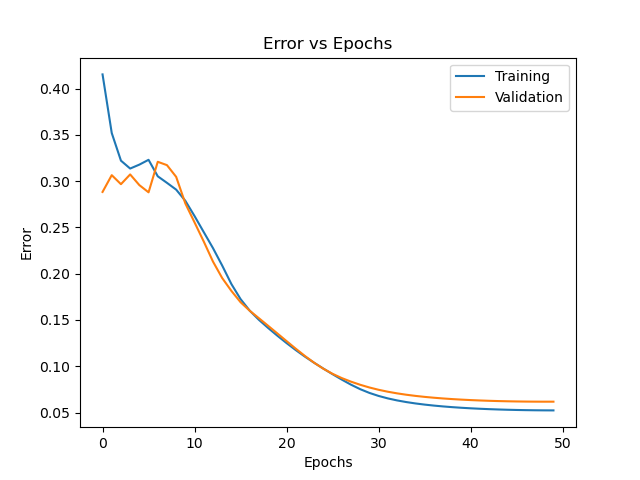
\includegraphics[scale = 0.5]{DataSet1ErrorPlot}
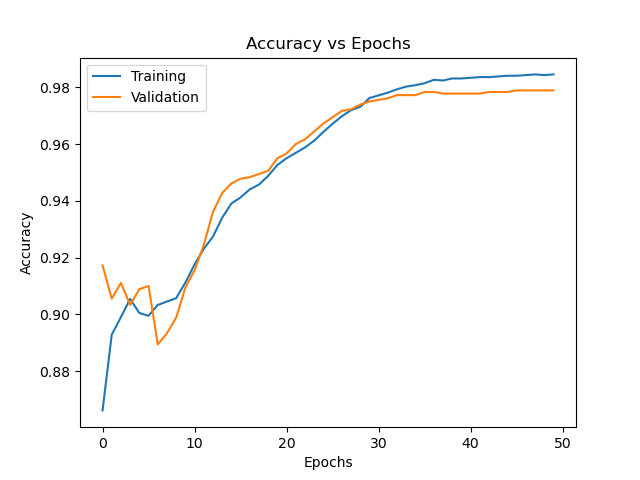
\includegraphics[scale = 0.5]{DataSet1AccuracyPlot}
\caption{Plot of the error vs epochs on DataSet1 (Left) and the plot of the accuracy vs epochs on DataSet1 (Right)}
\end{figure}

\begin{figure}[H]
\centering
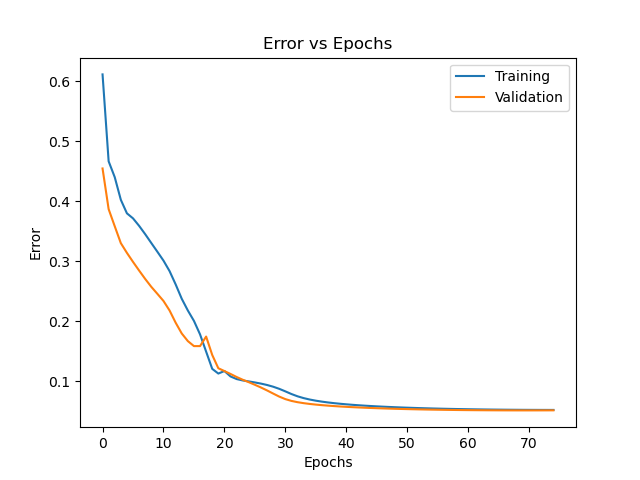
\includegraphics[scale = 0.5]{DataSet2ErrorPlot}
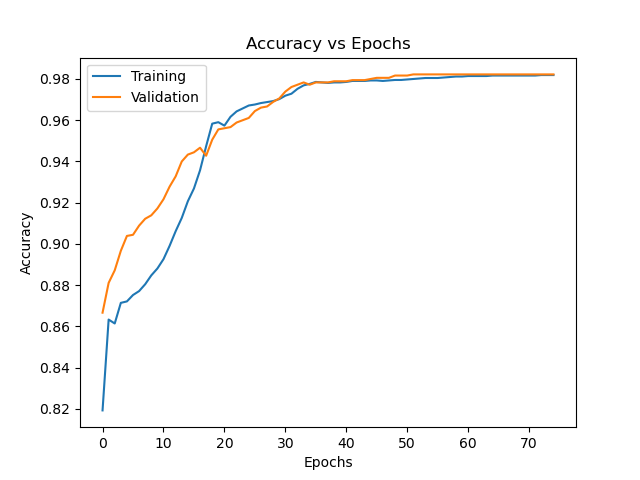
\includegraphics[scale = 0.5]{DataSet2AccuracyPlot}
\caption{Plot of the error vs epochs on DataSet2 (Left) and the plot of the accuracy vs epochs on DataSet2 (Right)}
\end{figure}

The error during both training decreased for both the training and validation datasets for both DataSet1 and DataSet2 (Figure 3).  The accuracy also increased during training for both DataSets as well (Figure 4).

\begin{figure}[H]
\centering
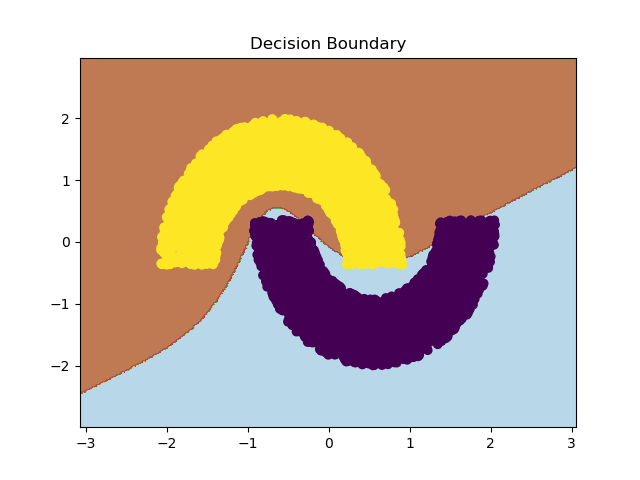
\includegraphics[scale = 0.33]{DataSet1BoundaryPlot}
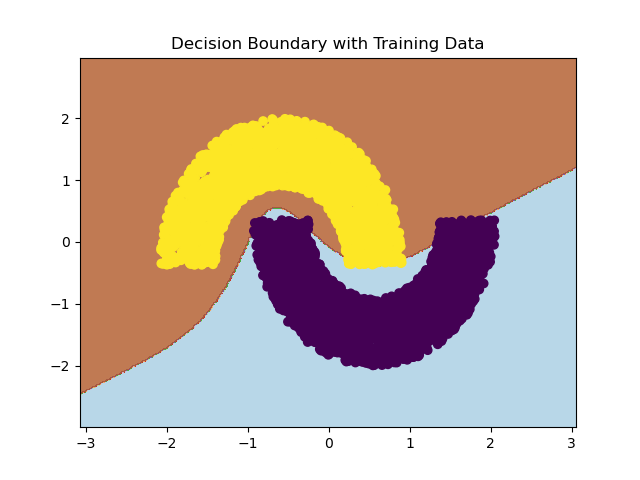
\includegraphics[scale = 0.33]{DataSet1TrainBoundaryPlot}
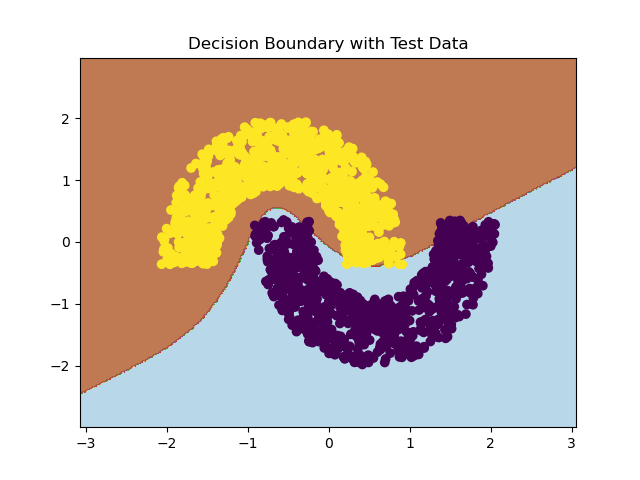
\includegraphics[scale = 0.33]{DataSet1TestBoundaryPlot}
\caption{Plot of the decision boundary for DataSet1 (Left), the plot of the decision boundary with only the training data for DataSet1 (Center), and the plot of the decision boundary with only the validation data for DataSet1 (Right)}
\end{figure}

\begin{figure}[H]
\centering
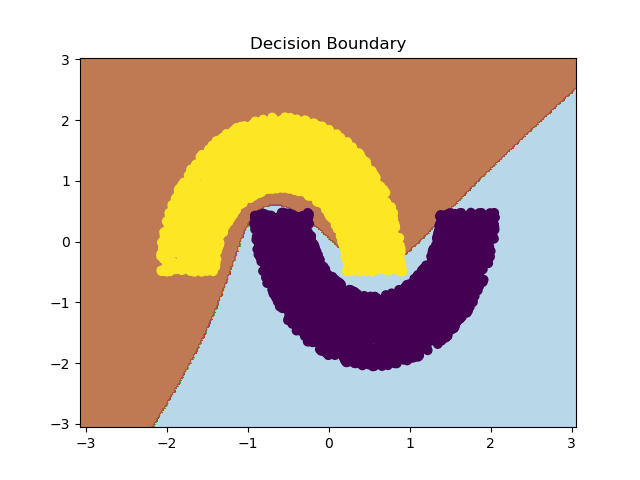
\includegraphics[scale = 0.33]{DataSet2BoundaryPlot}
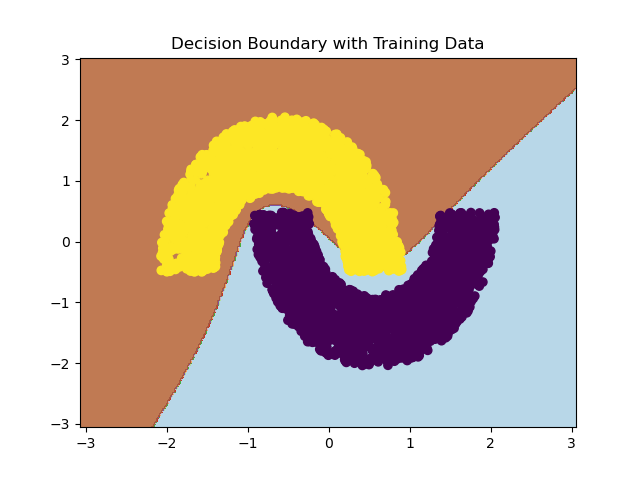
\includegraphics[scale = 0.33]{DataSet2TrainBoundaryPlot}
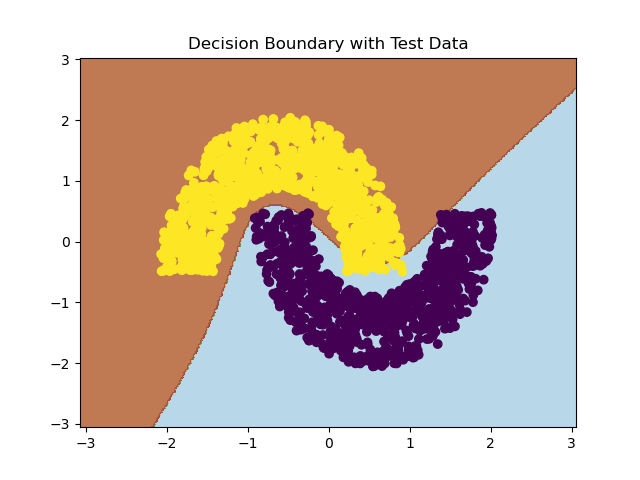
\includegraphics[scale = 0.33]{DataSet2TestBoundaryPlot}
\caption{Plot of the decision boundary for DataSet2 (Left), the plot of the decision boundary with only the training data for DataSet2 (Center), and the plot of the decision boundary with only the validation data for DataSet2 (Right)}
\end{figure}

We also plotted the decision boundaries for the full data sets as well as for the training and testing data individually. The decision boundary for DataSet1 is shown in Figure 5, and shows that the MLP was able to learn the data quite well. The same is true for DataSet2 in Figure 6. The miscalssified points are all near the decision boundary, and would likely have been classifeid correctly if the MLP had more parameters and flexibility to learn the data points.

\end{document}
